\chapter{Introduction}

\section{General motivation and objectives}

When natural disaster occur, a prompt intervention is a key factor. In order to organize effective rescue missions, it is fundamental to quickly gather information about collapsed buildings, damaged roads and, above all, victims. To this extent, autonomous Micro Aerial Vehicles (MAVs) are a promising technology to survey the stricken area.

The introduction of unmanned aerial vehicles (UAVs) has revolutionized military operations all over the world. In the past year, the U.S. reached an important milestone in that Air Force now has more UAVs than manned aircraft, while Israel and the United Kingdom had recent significant advances in UAV heavy-lift capacity \cite{6099676}. These advances are not only limited to the military as the international civil sector also looks to such unmanned technologies to aid operations such as fighting forest fires, undersea exploration, monitoring wildlife, inspecting bridges, and supporting first responders such as police and rescue organizations. UAV expenditures alone are predicted to more than double in the next ten years, and are expected to exceed \$80 billion \cite{6099676}.
So far this century there have been more than 1000 fatal earthquakes causing a total loss of life exceeding 1.5 million people. Reducing the loss of life is the primary priority of most earthquake protection strategies, and yet the processes that contribute to death tolls and the best strategies for reducing injury levels are not well understood. According to \cite{coburn1994death}, structural collapses are responsible for 75\% of deaths in earthquakes. The factors influencing the number of victims per building collapse fall into five major categories M1 to M5. Being M3 the “occupants trapped by collapse”.

In all three cases it’s evident how a flying vehicle can be useful to reach the areas struck by the earthquake. When disasters such as this occur, a prompt intervention is a key factor: the probability of saving lives decreases dramatically after the initial hours. In order to organize effective rescue missions, it is fundamental to quickly gather information about collapsed buildings, damaged roads and, above all, victims. To this extent, autonomous Micro Aerial Vehicles (MAV) are a promising technology to survey the stricken area. 
These applications usually require complete autonomy in navigation, small size of the air vehicle to access also confined out and indoor spaces and low power consumption for extended operation times. 


In the framework of swarm robotics involved in search and rescue (SAR or S\&R) applications, the main purpose of this thesis research is to investigate complete coverage algorithms. These kind of algorithms are intended in the first place to perform a fast monitoring by means of aerial imaging, but many other applications are possible.

The branch of swarm robotics is relatively new, and the application of swarm robotics to flying vehicles is even more innovative. The capacity of having multiple robots with such mobility in fact opens new possibilities with respect to terrain exploration.

I developed in parallel two different approaches: real-time and optimised coverage. They fit different hardware and swarm-type requirements, but they share the same mathematical base, graph theory.

To test the algorithms a 3D simulation environment was created and the simulated robots are controlled using the ROS robotic platform. This was mandatory choice for testing online algorithms, but nevertheless a good way to visualise the results for pre-processed optimised coverage.
The simulated environment has been represented as a graph using a convention shown in the next chapter, on which the algorithms operate to perform the coverage. As a last step the algorithms were also tested with success on a pair of real multi-copters available in the laboratory, proving that a consistent framework is available for immediate application.


\section{The Coverage Problem}

This thesis work deals with the problem of finding the most effective algorithm to solve the coverage problem. Let's then start defining what the coverage problem deals with and how we can solve it.

 The are two major classes in which we can divide coverage problems: \emph{static} coverage and \emph{dynamic} coverage. Given a finite area with obstacles to cover, the static coverage solves the problem of finding the best robot positions such that visibility of the area is maximized. In this case then there will be some which will not be monitored by the robots (blind spots) and for our SAR purposes this is unacceptable. For this reason in the thesis we opted for a dynamic approach to coverage. In a dynamic coverage the robot will have to cover the area by exploring it thoroughly, so even if at each time step we just observe a little portion of the terrain, the final knowledge of the area is complete. If for example we have to find a victim in a stricken environment and the person is hidden in a blind spot, the static coverage does not ensures that the victim will be detected, while the dynamic coverage does. A static coverage moreover does not observe the area uniformly; the regions near to the robot will be well monitored while far one will be observed only marginally.
 
Now in the the field of dynamic coverage we can identify two classes:
\begin{itemize}
\item \textbf{Offline coverage}: the paths are pre-calculated with a routing algorithm, before the robot start exploring the environment
\item \textbf{Online coverage}: the robots decide their path while they are exploring the environment, by making decisions based on the current knowledge they have on the coverage completion
\end{itemize}

An important aspect to take into account is whether the coverage is meant to be performed by a single robot, or by a group of robots. The main difference between the two is that in the single robot the robot does not have to interact with other moving units and this simplifies the planning and does not require a inter-robot communication system. In the multi-robot coverage instead the communication between units is essential to take advantage of a collaborative behaviour. In this thesis the main objective has been to build a flexible software framework that can  be easily extend from a single-robot to multi-robot configuration seamlessly.

For known environments it is important to accomplish the coverage task in the minimum possible time and using this a priori knowledge we can construct an algorithm that computes the optimal paths to completely cover the area. This is possible decomposing the environment in a finite number of spots to visit (see next section, \ref{sec:spaceDec}) and by modelling the coverage as a routing problem where we have to visit all the location at least once. But using offline algorithms to find optimal path turns out to be not so trivial, optimal solution are really hard to compute, actually NP-hard \cite{wiki:VRP}, so in practice heuristic and deterministic methods have been developed that find acceptably good solutions for the VRP. This involves a discrete computation capability and in the perspective of using the algorithms to guide autonomous robots this can represent a limitation. That is why several online strategies have also been investigated.
From a computational point of view online algorithms are far less challenging. In an online coverage basically the robot has the only simple task of choosing what step to take next, basing is decision of the current knowledge it has on the current level of completion of the coverage. It also has the advantage of being more flexible; think of a situation where a robot fails due to a crash: in an offline coverage the path are pre-calculated so the path assigned to that robot will not be covered, in an online case instead the robots will continue exploring the area till they know that the whole area is covered. They also fit better the swarm robotics approach where complex behaviours emerges from the sum of many simple ones.

As a final remark since performing SLAM (simultaneous localization and mapping) is out of the scope of this thesis the terrain is assumed to be known. Having in mind that by using any modern web mapping service the topology of the area can be retrieved this can be a reasonable assumption in real world applications.

The path planning required to perform the complete coverage task must be build on top of an abstract representation of the terrain. This abstract representation can be obtained through one of the various methods discussed in the next section.



\section{State of the art}

Many works have been present in the area of research dealing with the coverage problem, either offline or online, aiming to accomplish static or dynamic coverage, using single or multi-robot approach, and assuming known and unknown environments. In this paragraph we will review some of the solutions found in literature as a starting point for the research developed in this thesis.


\subsection{Coverage algorithms}

Regarding static coverage, in \cite{5152815} is presented a distributed control strategy for deploying hovering robots with multiple downward facing cameras to collectively monitor an environment. Information per pixel is proposed as an optimization criterion for multi-camera placement problems  to derive a specific cost function for multiple downward facing cameras. The cost function leads to a gradient-based distributed controller for positioning the robots, experimented with three AscTec Hummingbird quad-rotor robots. Although some works have been presented previously, in which a Voronoi partition of the environment is involved, this approach on the contrary relies on the fields of view of multiple cameras to overlap with one another.

A novel approach to static coverage is presented in \cite{5649249} where propose a cooperative algorithm to maximize the monitored areas in a 2D non-convex environment, by using a team of mobile robots. In particular, it deals with the maximization of an area monitored by a team of robots using vision sensors. A learning strategy is presented, able to provide a coordinated control algorithm for all the team members. In particular, the proposed approach is based on the Cognitive-based Adaptive Optimization (CAO) methodology.

Usually, regarding dynamic coverage, to find optimal paths using an offline algorithm most of the works in literature model the problem as one of the following one: \emph{Travelling Salesman Problem}, \emph{Chinese Postman Problem}, \emph{Watchman route problem} or \emph{Vehicle Routing Problem}. All of them aim to find the shortest path to cover all the vertices of a given graph by minimizing the travelled distance, but they slightly differ for the constraint they impose on the travelled path.

In \cite{ChongCoverage} the space decomposition problem is firstly analysed and then, after developing a recursive strategy for completely visit a set of connected rooms, a \emph{parallel swath} is used to perform the complete coverage of a single room, which consists in a simple back and forth exploration as shown in Fig. \ref{fig:covTypes}.

In \cite{navidCovAlgs} a series of coverage patterns are considered among which: parallel swath, contour swath with inward shift, random walk and outward spiral. In this work is claimed however that this kind of paths are not feasible for nonholonomic car-like vehicle due to the fact that the trajectories contain
discontinuities in the heading which requires the vehicle to turn on the spot, but since we are using micro aerial vehicles this constraint does not apply. This work also addressed the problem of covering occasional gaps and the \emph{Travelling Salesman Problem} (TSP) is proposed as a solution imposing the constraint that the generated paths to the uncovered areas should be as short as possible to minimize overlapped coverage.

\begin{figure}[ht]
\centering

\includegraphics[width=0.7\textwidth]{various_coverages_1}
\caption{Various dynamic coverage patterns}
\label{fig:covTypes}
\end{figure}

In \cite{MannadiarR10} a new algorithm based on the Boustrophedon cell decomposition is introduced. The presented algorithm encodes the areas (cells) to be covered as edges of the Reeb graph. The primary contribution of their algorithm is using the solution to the CPP in order to find the optimal order, in terms of distance travelled, in which the cells are covered. Then, given the Reeb graph an \emph{Euler tour} is calculated, that is a circuit that covers every edge in a graph exactly once. To cover the interior of a the cell a simple back-and-forth motion is used. The experiments were carried out by simulating a Pioneer robot to perform coverage of all the available free space, in different classes of environments as test cases.

In \cite{Naftos:1992} the \emph{Watchman Route Problem} (WRP) is investigated, that is: find a shortest route such that each point in the polygon $P$ is $d$-visible (i.e., visible and at most $d$ away) from some point along the route. For simple polygons when there is a visibility range $d$ and we are interested in viewing the whole interior of $P$. Two versions of the WRP are presented: find a shortest route such that either \emph{(a)} each point in the boundary of the polygon (d-watchman problem) or \emph{(b)} each point in the polygon ($d$-sweeper problem), is $d$-visible. An approximation algorithm for the TSP in simple grids is proposed, that obtains solutions within 33\% of the optimum. This also provides approximate solutions for the $d$-sweeper problem.

For the class of online algorithms, the most common approaches will be discussed  in greater detail in the body of the thesis, but let's firstly go briefly through all of them.
The simplest online algorithm is the so called \emph{Node Counting}. Basically this algorithm counts the number of visits in the various positions of the terrain to be covered and at each step chooses to go to the location with the smaller number of visits.

In \cite{Ishida:1998:RSA:608597.608621} can be found a good review of the \emph{LRTA*}. The logic behind this algorithm is similar to the Node Counting one, but in this case the value associated to a map position is not just its visit count but a cost value that is used to guide the robots near the unvisited locations. For a comparison between Node Counting and LRTA* see \cite{koenig2001}.

In \cite{Koenig96easyand} the \emph{Edge Counting} algorithm is presented. In this case the count used for making decisions is the edge traversal count of the departing links, from the current position, to the next reachable ones. Random walks are bad search algorithms since they do not remember were they have already searched but it be can easily derived a real-time search algorithm that shares many properties with random walks, but has finite complexity - basically, by “removing the randomness” from random walks. In \cite{506507}, is proved that edge counting always reaches a goal state with a finite number of action executions, but its complexity can be exponential in the size of the state space.

In \cite{5711675} the \emph{PatrolGraph*} algorithm is introduced. It takes into account both the number of visits and as node count and the edge traversals. The algorithms has been specifically designed to solve the problem of Multi–Robot Controlled Frequency Coverage (MRCFC), in which a team of robots are requested to repeatedly visit a set of pre–defined locations of the environment according to a specified frequency distribution. It is proven to
be statistically complete as well as easily implementable on real, marketable robot swarms for real–world applications.In this thesis we will exploit the properties of this algorithm to perform a Multi–Robot Uniform Frequency Coverage (MRUFC), so that all the locations of the map will be visited uniformly.


\subsection{Space Decomposition}
\label{sec:spaceDec}

To perform a path planning and define a metric for deciding when a coverage is complete we have to sub-sample the space using a methodical approach. The most common approach is to apply a so called \emph{cellular decomposition} to the space. A mathematical definition of cellular decomposition is given in definition \ref{cellDec}.

\theoremstyle{definition}
\begin{definition}{\textbf{\textit{Cellular decomposition}}}\label{cellDec}
In geometric topology, a cellular decomposition $G$ of a manifold $M$ is a decomposition of $M$ as the disjoint union of cells (spaces homeomorphic to n-balls $B_n$).
\end{definition}

Practically a cellular decomposition is a data structure that encodes the topology of a given environment, using elementary non-overlapping regions of terrain of known geometry such that adjacent cells share a common boundary and that the union of all cells coincides with the environment. The main purpose of the decomposition is to derive an abstract description of the free space, i.e., the one in which the robot can move. Moving from cell to cell and covering the space in each cell for all of them will result in covering the entire region.
\clearpage
\noindent We can distinguish two types of cellular decomposition:
\begin{enumerate}
\item Exact cell decomposition (topology-dependent)
\item Approximate cell decomposition (topology-independent)
\end{enumerate}


In the exact cell decomposition the topology of the environment is accurately represented and to accomplish this all the cells does not have to be the same size, but they contain only free space. The method also requires a complete description of the objects and a complex cell construction.  In approximate cell decomposition, the entire region is divided into equal sized cells. Any cell with any part of an obstacle in it is marked as invalid workspace. The cells do not necessarily have to be marked as empty or full, but can be represented by a fraction of the portion occupied. The approximation can be improved by increasing the resolution but this of course will increase the memory requirements if the entire grid is stored in memory. After the cells are created an adjacency graph can be produced where each vertex represents a cell and the edges represents the adjacency relationship between the cells. Then this adjacency graph is used by the algorithms to perform the path planning in order to complete the coverage.

In \cite{846365} the authors present some new examples of exact cellular decompositions whose cells are defined by critical points of Morse functions. Cellular decompositions have been widely used for planning a path between two points in the free space, but the motivating task for the work presented in this paper is coverage. Since the Morse functions define cells with “simple” structure, a planner can then use a cellular decomposition to achieve coverage by employing simple control strategies to cover each of the individual cells in the decomposition. A simple
control strategy can be back-and-forth motions, resulting in a farming style pattern.

\begin{figure}[t] 
  \label{fig:cellDec_typess} 
  \begin{minipage}[b]{0.5\linewidth}
    \centering
    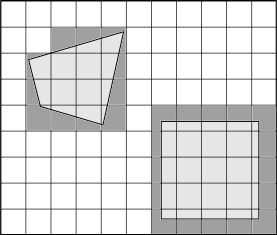
\includegraphics[width=0.7\textwidth]{approx_cell_decomp}
    \caption{Approx. cell decomposition}
    \label{fig:cellDec_pic1}
    \vspace{4ex}
  \end{minipage}
  \begin{minipage}[b]{0.5\linewidth}
    \centering
    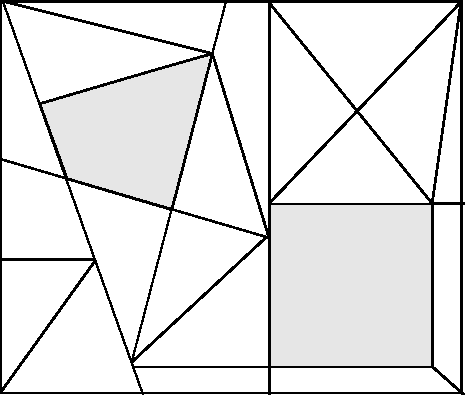
\includegraphics[width=0.7\textwidth]{exact_cell_decomp}
    \caption{Exact cell decomposition}
    \label{fig:cellDec_pic2}
    \vspace{4ex}%%
  \end{minipage}
  \begin{minipage}[b]{0.5\linewidth}
    \centering
    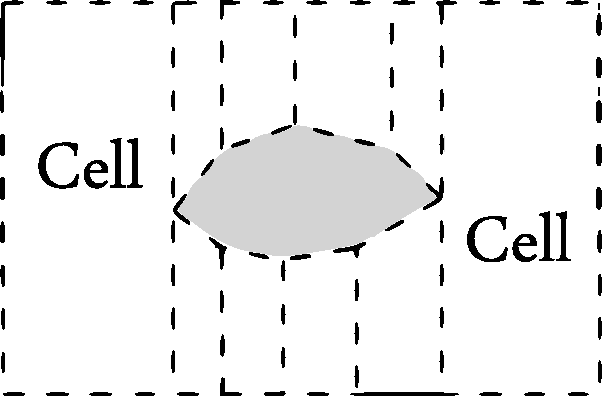
\includegraphics[width=0.7\textwidth]{trapezoidal_1}
    \caption{Trapezoidal decomposition} 
    \label{fig:cellDec_pic3}
    \vspace{4ex}
  \end{minipage}
  \begin{minipage}[b]{0.5\linewidth}
    \centering
    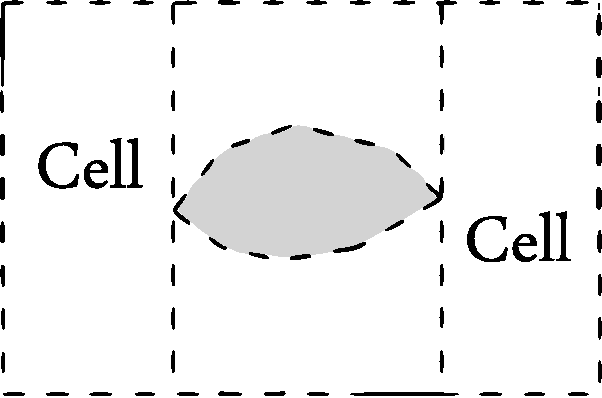
\includegraphics[width=0.7\textwidth]{boustrophedon_1}
    \caption{Boustrophedon decompostion}
    \label{fig:cellDec_pic4}
    \vspace{4ex}%% 
  \end{minipage} 
\end{figure}

In \cite{choset} the Boustrophedon Cellular Decomposition is introduced (figures \ref{fig:cellDec_pic3} and \ref{fig:cellDec_pic4}). Is an exact cellular decomposition approach, for the purposes of coverage. Essentially, the boustrophedon decomposition is a generalization of the trapezoidal decomposition that could allow for non-polygonal obstacles, but also has the side effect of having more “efficient” coverage paths than the trapezoidal decomposition. Cells are formed via a sequence of open and close operations which occur when the slice encounters an event, an instance in which a slice intersects a vertex of a polygon. There are three types of events: \emph{in}, \emph{out}, and \emph{middle}. Loosely speaking, at an \emph{in} event the current cell is closed (thereby completing its construction) and two new cells are opened (thereby initiating their construction). The boustrophedon cellular decomposition is an enhancement of the trapezoidal decomposition and is designed to minimize the number of excess lengthwise motions, as described in the previous paragraph. In essence, all cells between \emph{in} and \emph{out} events are merged into one cell. The advantage of having a fewer number of cells is that to complete the coverage the number of back-and-forth boustrophedon motions can be minimized. 

\begin{figure}[t] 
  \label{fig:grid_types} 
  \begin{minipage}[b]{0.5\linewidth}
    \centering
    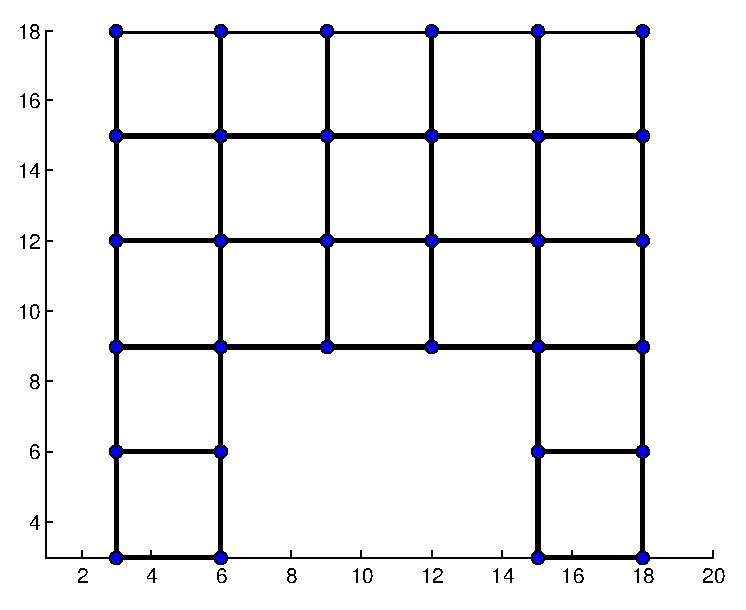
\includegraphics[width=0.7\textwidth]{6x6_Sparse1_1}
    \caption{Simple grid}
    \label{fig:grid1}
    \vspace{4ex}
  \end{minipage}
  \begin{minipage}[b]{0.5\linewidth}
    \centering
    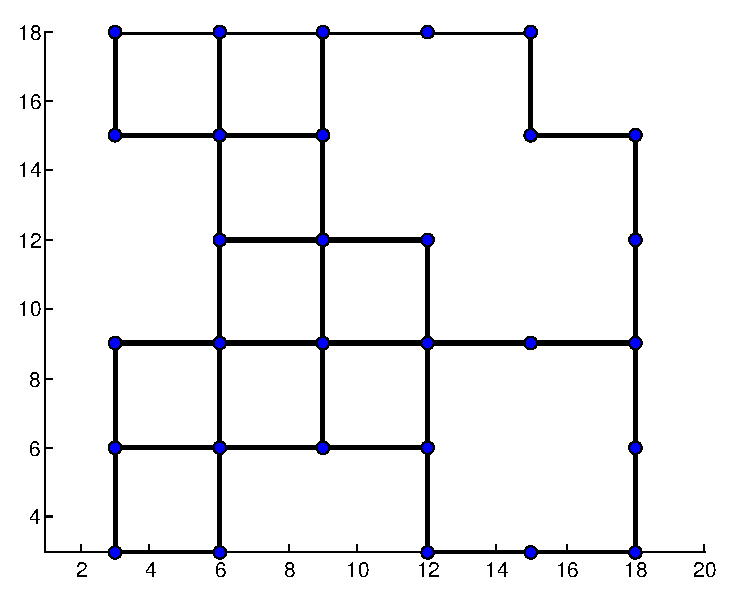
\includegraphics[width=0.7\textwidth]{6x6_Sparse2_1}
    \caption{Non-simple grid w/o l.c.n.}
    \label{fig:grid2}
    \vspace{4ex}%%
  \end{minipage}
\end{figure}

Regarding the approximate cell decomposition instead the logic is much simpler, since the only decision we have to make is how much we want the grid to be detailed. Then we mark as free only the cells that not contain any obstacle and all the rest as non-accessible space. In \cite{stanf:cellDec} a recursive strategy is presented where the cells are continuously subdivided until one of the following scenarios occurs: each cell lies either completely in free space or completely in the C-obstacle region, an arbitrary limit resolution is reached.
Once a cell fulfils one of these criteria, it stops decomposing. This method is also called a \emph{quadtree decomposition} because a cell is divided into four smaller cells of the same shape each time it gets decomposed.

Among the resulting grids we can distinguish between \mbox{\textit{simple grids}} (i.e., without internal holes) and \textit{non--simple grids} which do not possess \textit{local cut nodes} (i.e., nodes whose removal locally disconnects the graph induced by the grid). 


Both exact cell decomposition methods and approximate cell decomposition methods have advantages and disadvantages. The former are guaranteed to be complete, meaning that if a free path exists, exact cell decomposition will find it; however, the trade-off for this accuracy is a more difficult mathematical process. Approximate cell decomposition is less involved, but can yield similar, if not exactly the same, results as exact cell decomposition.







\section{Terminology and Notation}\label{sec:terminology}

Due to the simultaneous use of the ROS network and graph theory, we will always try to use two distinct names when referring to nodes and vertices. In particular in the ROS environment is formed of nodes and a graph has vertices.

That said, every terrain can be modelled as a undirected graph, by sampling the area using a grid.
The grid is described by a navigation graph $G_N=(V,E)$, the \emph{navigation graph}, where $V$ is a set of vertices and $E$ is a set of edges. Each edge that connects vertex $i$ to vertex $j$ is represented as $e_{ij}=e(i,j)$. Let be $N(v)$ the set of vertices adjacent (connected through an edge) to $v$. The maximum degree (number of edges incident to a vertex) of the graph $G$ will be denoted by $\Delta (G)$ and the minimum degree by $\delta (G)$.


\theoremstyle{definition}
\begin{definition}{\textbf{\textit{Eulerian State Spaces}}}\label{cellDec}
A state space is Eulerian if  there are as many actions  that leave a state as there are actions that enter the (same) state.
\end{definition}

Since an undirected edge is equivalent to one incoming and one outgoing edge, all undirected state spaces are Eulerian.

The navigation graph is better represented through a strongly connected, oriented graph $\hat{G}_N$, derived from $G_N$ by doubling all its edges and assigning them opposite directions. 
$E_i=\{e_{ij}\} \neq 0$ is the finite, nonempty set of directed edges that leave vertex $v_i \in V$.  $|E_i|$ is the dimension of the set, i.e., the number of edges departing from $v_i$.

$R=\{r_i\}$ is a set of $M$ robots. Robots are allowed to move in the workspace from $v_i$ to $v_j$ in $\hat{G}_N$ only if $e_{ij} \in E_i$, i.e., if the two vertices are adjacent. 
${\bm{\lambda}}=[\lambda_1,\cdots,\lambda_N]^T  \in \Re^N$ is a vector which describes the average visiting rate to each vertex $v_i \in S$, expressed as \textit{number of robots} per \textit{time unit}. %\Re$).
${\bm{\lambda}}^*=[\lambda_1^*,\cdots,\lambda_N^*]^T  \in \Re^N$, $0 \le \lambda_i^* \le 1$ and $\sum \nolimits_1^N \lambda_i^* =1$ is a vector which describes the prescribed frequency distribution of visits. 

Similarly to \cite{koenig2001}, the expression ``one-of $X$'' returns randomly one of the elements of $X$. The notation $succ(v,e)$ returns the vertex linked to $v$ through the edge $e$. The expression $c(v)$ represents the count value associated with to the vertex $v$, initially set to zero for all $v \in V$.

Let be $U$ a structure containing all the vertices of the graph still to be visited, i.e., the \emph{unvisited set}. At last let $\ell(\cdot)$ be the function that returns the length of a path and, in particular, let $\ell(P_i) \equiv \ell_i$ be the length of the $i-$th path.














